\documentclass[9pt,compress]{beamer}

% ========================================================
% CUSTOMIZATIONS 
\newcommand{\authorname}{First Name Last Name}
\newcommand{\shortauthor}{R. Sanchez}
\newcommand{\authoremail}{first.last@c137.com}
\newcommand{\coauthors}{Co-author1, Cco-author2}
\newcommand{\institution}{Some University}
\newcommand{\authoraffiliation}{Some lab}
\newcommand{\slidesettitle}{Smart, concise and short title}
\newcommand{\shorttitle}{Short title}
\newcommand{\slidesetsubtitle}{}
\newcommand{\logoimagepath}{logos/poly_logo}
\newcommand{\logoimagepathlab}{logos/lm2_logo}

% ==========================================================
%% PACKAGES
\usepackage[utf8]{inputenc}
%\usepackage[english]{babel}
\usepackage[english]{babel}
\usepackage{tikz}
\usepackage{adjustbox}
\usepackage[T1]{fontenc}
\usepackage{graphicx}
\usepackage{tikz}
\usepackage{textpos}
\usepackage{color}
\usepackage{etex}
\usepackage{cite}
\usepackage{rotating}
\usepackage{hyperref}
\usepackage{import}
\usepackage{media9}
\usepackage{subfig}
\DeclareCaptionLabelSeparator{horse}{:\quad} % change according to your needs
%\captionsetup{labelsep = horse,figureposition = bottom} 
\usepackage{textcomp,amsfonts,stmaryrd,soulutf8}
\usepackage{xifthen}% provides \isempty test
\usepackage{longtable,ifthen,xspace,url}
\usepackage{verbatim,pdflscape}
\usepackage[babel=true]{csquotes} % style de guillements 
\usepackage{bibentry}
\bibliographystyle{ieeetr}
%\usepackage{lipsum}
\usepackage{caption}
\captionsetup{font=scriptsize,labelfont=scriptsize}

\graphicspath{{./images/}}

%% Maths
\usepackage{mathtools,mathabx,mathpazo}
\usepackage{amsmath,amssymb,amscd,mathrsfs,fixmath}
%fraction a/b
\newcommand{\rfrac}[2]{\raisebox{0.5ex}{$#1$}\slash\raisebox{-0.5ex}{$#2$}} 
% function f->...
\newcommand{\function}[5]{\begin{array}{crcl}
#1 \, : & #2 & \longrightarrow & #3 \\
    & #4 & \longmapsto & #5 \end{array}}
%\begin{equation}
%\function{d}{\mathbb{R}^3}{\mathbb{R}^3}{\boldsymbol\xi}{\boldsymbol{d}(\boldsymbol\xi) = \boldsymbol\eta}  
%\end{equation}

% ==========================================================
%BEGIN DOCUMENT
%\begin{document}
% ==========================================================
% DO NOT MODIFY THE NEXT LINE
% First slide + template
\usetikzlibrary{decorations.fractals}
\useoutertheme[subsection=false,shadow]{miniframes}
\useinnertheme{default}
\usefonttheme{serif}
\usefonttheme{professionalfonts}
\useoutertheme{infolines}

%POLYMTL COLORS
\definecolor{polyblue}{HTML}{41AAE6}
\definecolor{polygreen}{HTML}{8CC83C}
\definecolor{polyorange}{HTML}{FA961E}
\definecolor{polyred}{HTML}{B91E32}
\definecolor{polygray}{HTML}{A6A8AB}

%SIDEBAR
\usetheme[hideothersubsections]{Goettingen}
\setbeamersize{sidebar width right=0.15\paperwidth}
\makeatletter
\setbeamertemplate{sidebar canvas \beamer@sidebarside}[vertical shading][top=polyred!15,bottom=polyred!10]
\makeatother
\usepackage{etoolbox}
\patchcmd\insertverticalnavigation{\dohead}{\vskip-25pt\dohead}{}{}

%%% TABLE Packages
\usepackage{array,multirow,makecell}
\setcellgapes{1pt}
\makegapedcells
\usepackage{colortbl}
\newcolumntype{R}[1]{>{\raggedleft\arraybackslash }b{#1}}
\newcolumntype{L}[1]{>{\raggedright\arraybackslash }b{#1}}
\newcolumntype{C}[1]{>{\centering\arraybackslash }b{#1}}
%Epaisseur lignes horizontales tableaux
\newlength\epaisLigne 
 \newcommand\Ghline{\noalign{\global\epaisLigne\arrayrulewidth\global
                              \arrayrulewidth 3pt}
		    \hline\noalign{\global\arrayrulewidth\epaisLigne}} 
 \newcommand\Mhline{\noalign{\global\epaisLigne\arrayrulewidth\global
                              \arrayrulewidth 1.5pt}
		    \hline\noalign{\global\arrayrulewidth\epaisLigne}}

% BEAMER TEMPLATE
\setbeamertemplate{caption}[numbered]
\setbeamertemplate{navigation symbols}{}

% Table of Contents
\setbeamertemplate{section in toc}[circle]
\setbeamerfont{section in toc}{shape=\bfseries\scshape, size=\large}
\setbeamerfont{footnote}{size=\tiny}
\setbeamerfont{caption}{size=\scriptsize}
\setbeamercolor{section number projected}{fg=white,bg=polyred}
\setbeamerfont{section number projected}{series=\bfseries, size=\normalsize}
\setbeamertemplate{subsection in toc}[square]
\setbeamercolor{subsection number projected}{bg=polyorange}

\setbeamerfont{frametitle}{shape=\bfseries\scshape}
\setbeamerfont{frametitle}{size=\LARGE}
\setbeamerfont{framesubtitle}{shape=\normalfont\bfseries}
\setbeamerfont{framesubtitle}{size=\normalsize}
\setbeamerfont{block title}{shape=\normalfont\bfseries}
\setbeamerfont{block title}{size=\normalsize}

\setbeamercolor{lower separation line head}{bg=DeepSkyBlue4} 
\setbeamercolor{normal text}{fg=black} 
\setbeamercolor{alerted text}{fg=polyred} 
\setbeamercolor{example text}{fg=black} 
\setbeamercolor{frametitle}{fg=polyred} 
\setbeamercolor{framesubtitle}{fg=polyorange} 
\setbeamercolor{structure}{fg=black} 
\setbeamercolor{palette tertiary}{fg=black} 
\setbeamercolor{palette quaternary}{fg=black} 
\setbeamercolor{block title}{fg=polyblue}

% HEADBARCOLOR FIRST SLIDE MASKED
\newcommand{\headbarcolor}{polyred}
\setbeamertemplate{headline}{% 
	\setbeamercolor{head1}{bg=\headbarcolor}
	\hbox{%
  \begin{beamercolorbox}[wd=.5\paperwidth,ht=0ex,dp=0ex,center]{head1}%
  \fontsize{5}{5}\selectfont
  
  \end{beamercolorbox}%
  }
  \vspace{-25ex}
}

% FOOT LINE / FOOTPAGE / FOOTNOTE
\newcommand{\footref}[1]{\textsuperscript{\ref{#1}}}
\let\Tiny=\tiny
\setbeamertemplate{footline}{
\begin{tiny}
\setbeamercolor{foot1}{fg=polyblue,bg=polyblue!10}
\setbeamercolor{foot2}{fg=polygreen,bg=polygreen!10}
\setbeamercolor{foot3}{fg=polyorange,bg=polyorange!10}
\setbeamercolor{foot4}{fg=polyred,bg=polyred!10}

% taken from theme infolines and adapted
  \leavevmode%
  \hbox{%
  \begin{beamercolorbox}[wd=.4\paperwidth,ht=2.25ex,dp=1ex,center]{foot1}%
	\shorttitle
  \end{beamercolorbox}%
  
  \begin{beamercolorbox}[wd=.2\paperwidth,ht=2.25ex,dp=1ex,center]{foot2}
	\shortauthor
  \end{beamercolorbox}%
  
  \begin{beamercolorbox}[wd=.25\paperwidth,ht=2.25ex,dp=1ex,center]{foot3}
	\authoremail
  \end{beamercolorbox}%
  
  \begin{beamercolorbox}[wd=.15\paperwidth,ht=2.25ex,dp=1ex,right]{foot4}%
	\insertframenumber{} / \inserttotalframenumber \hspace*{2ex} 
  \end{beamercolorbox}}%
  
  \vskip0pt%
\end{tiny}
\vskip2pt
}

% HIDE SIDEBAR FIRST SLIDE
\newenvironment{specialframe}
{
    \begingroup
    \advance\textwidth1.6cm % see beamerthemeGoettingen.sty for the number
    \hsize\textwidth
    \columnwidth\textwidth
    \begin{frame}[plain]
}
{
    \end{frame}
    \endgroup
}

% %%%%%%%%%%%%%%%%%%%%%%%%%%%%%%%
% PDF INFO

\hypersetup{
  pdftitle={\slidesettitle},
  pdfauthor={\authorname},
  pdfstartview={Fit},
  colorlinks=true,            % colorise les liens
  breaklinks=true,            % permet les retours à la ligne pour les liens trop longs
  urlcolor=black,             % couleur des hyperliens
  linkcolor=black,            % couleur des liens internes aux documents
  citecolor=black             % couleur des liens vers les references
}

% %%%%%%%%%%%%%%%%%%%%%%%%%%%%%%% 
% FIRST SLIDE TEMPLATE
%\title{\slidesettitle}
%\subtitle{\slidesetsubtitle}
%\author{\authorname}

\begin{document}
%\tracingall
%\nobibliography{Biblio}

{\setbeamertemplate{footline}{}
	\begin{specialframe}
	%\begin{minipage}[c]{1.0\linewidth}
      	\includegraphics[height=15mm]{\logoimagepathlab}
      	\hfill
		\includegraphics[height=15mm]{\logoimagepath}
   	%\end{minipage}		

\begin{center}
{\Huge \textcolor{polyred}{\textbf{\scshape{\slidesettitle}}}} \\
\vspace{5pt}
\normalsize{\textcolor{polyorange}{\textbf{\slidesetsubtitle}}}
\end{center}

\begin{block}{}
			\begin{columns}
				
				\column{0.1\textwidth}
							
				\column{0.4\textwidth}				
				\newline \\	
				\normalsize{\textbf{\authorname}} \\
				{\footnotesize \textit{\coauthors}} \\
				{\footnotesize \authoremail} \\
				\vspace{15pt}
				{\footnotesize \authoraffiliation \\ \institution}\\				\vspace{15pt}
				{\footnotesize \textcolor{gray}{\insertdate}}
				
				\column{0.5\textwidth}
				\begin{figure}
					\centering
					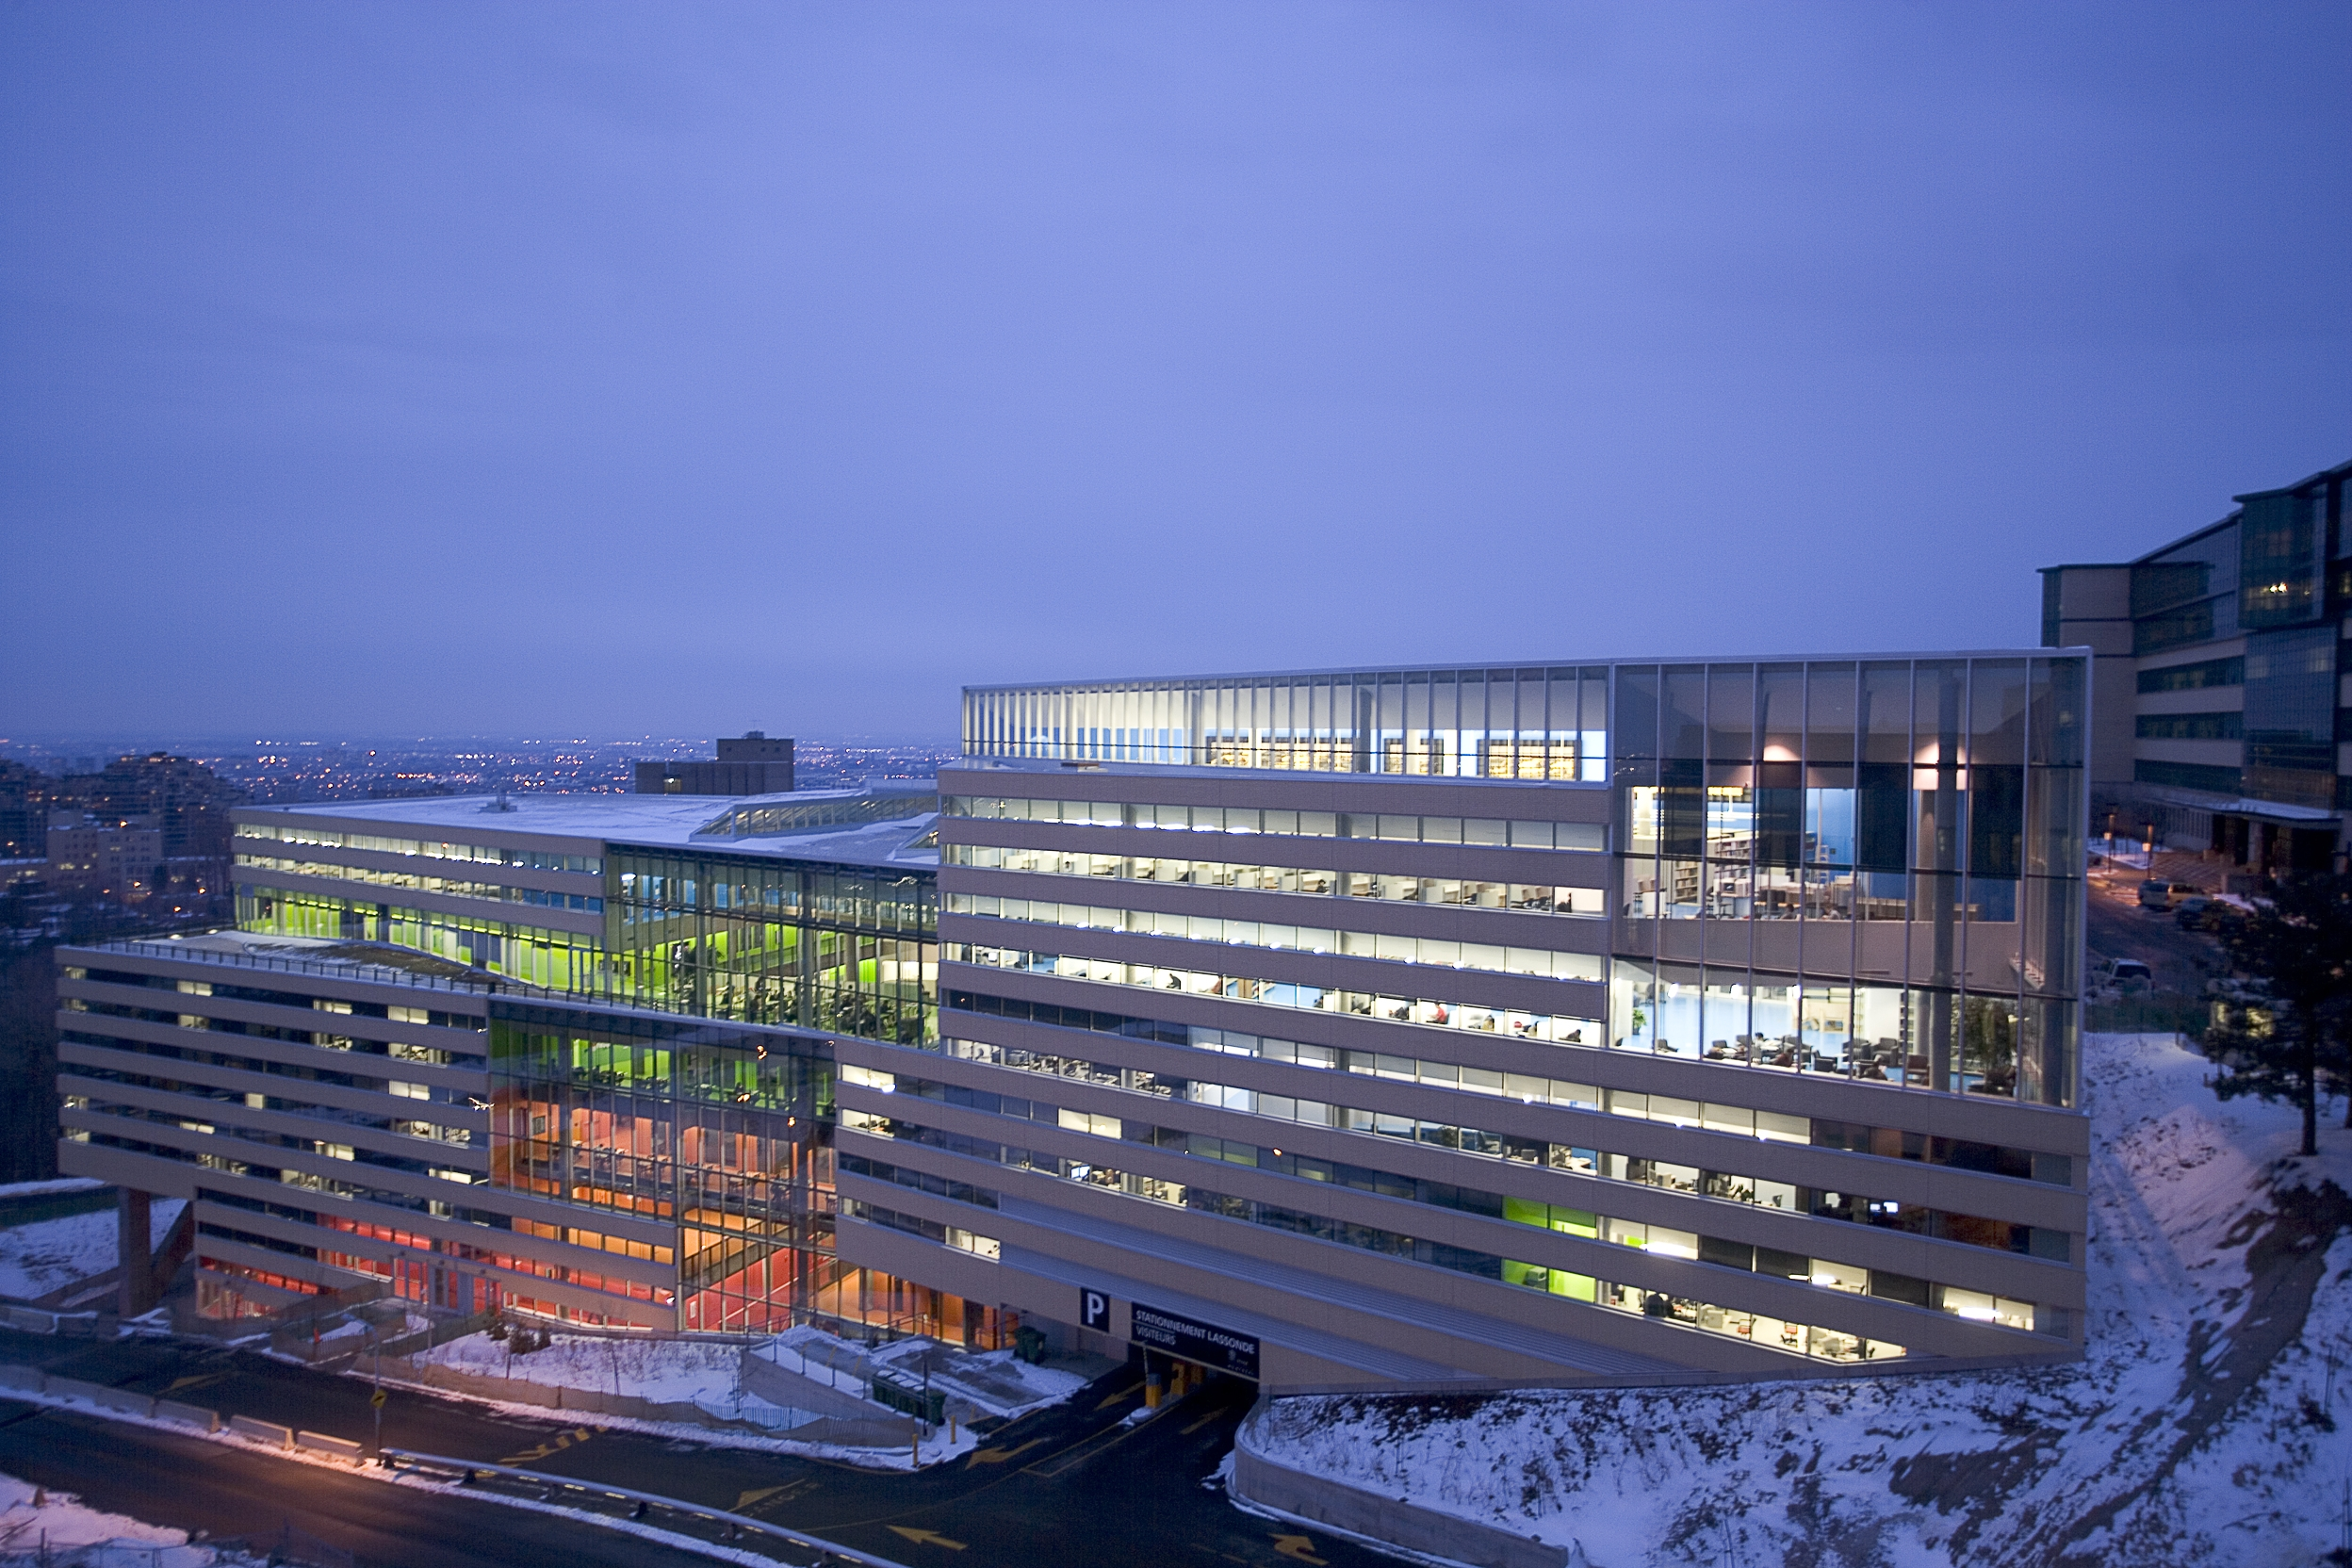
\includegraphics[width=0.95\textwidth]{logos/polytechnique.jpg}
				\end{figure}
				
			\end{columns}
		\end{block}

%\lipsum
\end{specialframe}
}

% %%%%%%%%%%%%%%%%%%%%%%%%%%%%%%% 
% OTHER SLIDES TEMPLATE

\setbeamertemplate{headline}{% 
	\setbeamercolor{head1}{bg=\headbarcolor}
	 \hbox{%
  \begin{beamercolorbox}[wd=.01\paperwidth,ht=2.25ex,dp=11ex,center]{head1}%
  \fontsize{5}{5}\selectfont
  \end{beamercolorbox}%
  }
  \vspace{-15.5ex}
	\begin{flushright}
		\includegraphics[height=5mm]{\logoimagepath} \\
		\vspace{1mm}
		\includegraphics[height=5mm]{\logoimagepathlab}

	\end{flushright}
}
% greater line spacing for new slides
%\linespread{1} 

% ======================= BEGIN SLIDES =====================
	
%Sets

\captionsetup{font=scriptsize, labelfont=scriptsize}


%=================================================================================================
%=================================================================================================
\section{Section}	
%=================================================================================================
%=================================================================================================
\subsection{Sub-section}	
%=================================================================================================
\begin{frame}
	\frametitle{Frame Title}
	\framesubtitle{Frame subtitle}

\end{frame}


\end{document}
